\scanpage{20}
Ainsi les classes de $\Pi_I^{\unsure{\circ|0}}$ sont les classes de $\Pi_J^\circ$ distinctes de $\deleted{\Pi}U_{J,i}$, et de plus les \unsure{clas|deux}. parmi
\[
U_{J,i}\cap
% BEGIN R020-G01
% First positive Sigma, complete glyph/index/plus. Origin (825,390), y down,
% baseline full y=450. Short separate head and curved upper arm each occur once.
% The first local qualifier covers the unresolved head role and index state.
% Complete index readings: deleted J followed by i | j | i. The separate
% short head is retained without assigning it a closure operation.
\mathord{\unsure{\begin{tikzpicture}[x=0.022em,y=-0.022em,baseline={(0,60)}]
\path[use as bounding box] (-3,0) rectangle (115,104);
\node[overlay,anchor=base west,inner sep=0pt,outer sep=0pt] at (0,60)
{\phantom{$\Sigma_{\unsure{\deleted{J}i|j|i}}^+$}};
\draw[line width=0.45pt,line cap=round] (7,15)--(49,11);
\draw[line width=0.55pt,line cap=round,line join=round]
 (7,21)..controls (37,22) and (45,24)..(45,34)
 --(10,58)..controls (27,57) and (44,54)..(58,54);
\draw[line width=0.35pt,line cap=round]
 (58,56)..controls (58,67) and (60,77)..(58,85)
 ..controls (45,90) and (29,94)..(22,91)
 ..controls (35,86) and (50,87)..(55,85)--(47,97);
\draw[line width=0.55pt,line cap=round]
 (58,54)..controls (59,59) and (58,65)..(60,67)
 ..controls (64,68) and (71,64)..(75,59);
\fill (66,39) ellipse (1.7 and 2.2);
\draw[line width=0.50pt,line cap=round] (84,17)--(102,15) (92,9)--(94,24);
\end{tikzpicture}}}
% END R020-G01
,\quad U_{J,i}\cap
% BEGIN R020-G02
% Paired negative Sigma, complete glyph/index/minus. Origin (1215,390),
% baseline full y=450. Same unresolved short-head role, recorded locally;
% the first occurrence above carries the page's recurring role qualifier.
\mathord{\begin{tikzpicture}[x=0.022em,y=-0.022em,baseline={(0,60)}]
\path[use as bounding box] (-3,0) rectangle (117,82);
\node[overlay,anchor=base west,inner sep=0pt,outer sep=0pt] at (0,60)
{\phantom{$\Sigma_i^-$}};
\draw[line width=0.45pt,line cap=round] (7,13)--(48,17);
\draw[line width=0.55pt,line cap=round,line join=round]
 (6,23)..controls (24,24) and (38,30)..(43,35)
 --(15,55)..controls (30,54) and (40,54)..(48,55)
 ..controls (53,56) and (56,60)..(55,67);
\fill (65,48) ellipse (1.7 and 2.0);
\draw[line width=0.50pt,line cap=round]
 (75,12)..controls (88,11) and (102,11)..(110,13)--(111,16);
\end{tikzpicture}}
% END R020-G02
\]
qui sont non vides. Or les deux classes en question sont non vides, car
$
% BEGIN R020-G03
% Cancelled Sigma before U, complete letter, j/i index and crossing strokes.
% Origin (315,805), baseline full y=875. Short head retained once.
% The qualifier records the local j/i and correction-state uncertainty.
% The repeated short-head role remains in the local doubt record.
\mathord{\unsure{\begin{tikzpicture}[x=0.022em,y=-0.022em,baseline={(0,70)}]
\path[use as bounding box] (-3,-2) rectangle (91,102);
\node[overlay,anchor=base west,inner sep=0pt,outer sep=0pt] at (0,70)
{\phantom{$\deleted{\Sigma_{\unsure{j|i}}}$}};
\draw[line width=0.45pt,line cap=round] (8,27)--(54,24);
\draw[line width=0.45pt,line cap=round,line join=round]
 (12,32)..controls (24,35) and (43,37)..(50,41)
 --(8,70)..controls (28,68) and (42,67)..(53,66);
\draw[line width=0.50pt,line cap=round]
 (64,78)..controls (64,83) and (64,89)..(67,89)
 ..controls (72,89) and (76,86)..(77,83);
\fill (73,31) ellipse (1.8 and 2.1);
\draw[line width=0.45pt,line cap=round]
 (8,68)--(41,10)--(39,13);
\draw[line width=0.45pt,line cap=round]
 (40,68)..controls (44,75) and (49,77)..(50,74)
 ..controls (57,60) and (62,43)..(67,32);
\end{tikzpicture}}}
% END R020-G03
$
$U_{J,i}$ est un voisinage
% A020-G02: gray detached round point, source origin (1175,817), baseline y=817.
% Shape candidate only; role, hand and surface origin unresolved. No word is in this group.
\unsure{\begin{tikzpicture}[baseline={(0,0)},x=0.025em,y=-0.025em]
\useasboundingbox (0,0) rectangle (11,24);
\fill[gray] (4,18) ellipse [x radius=2.2,y radius=2.5];
\end{tikzpicture}}
de $\deleted{\Sigma}E_{\unsure{i|j}}$, et
\[
% BEGIN R020-G04
% First barred positive Sigma, complete long outer rule, separate short head,
% curved main arm, lower body/index and raised plus. Origin (290,925),
% baseline full y=1005. The long closure bar is already present in C and H.
% The separate shorter head's role stays unresolved; it is drawn literally.
\mathord{\begin{tikzpicture}[x=0.022em,y=-0.022em,baseline={(0,80)}]
\path[use as bounding box] (-3,0) rectangle (117,103);
\node[overlay,anchor=base west,inner sep=0pt,outer sep=0pt] at (0,80)
{\phantom{$\overline{\Sigma_i^+}$}};
\draw[line width=0.35pt,line cap=round] (13,17)--(110,12);
\draw[line width=0.50pt,line cap=round] (7,35)--(58,27);
\draw[line width=0.55pt,line cap=round,line join=round]
 (15,39)..controls (47,39) and (56,44)..(51,51)
 --(10,79)..controls (30,78) and (50,76)..(65,76)
 ..controls (70,76) and (73,80)..(71,84)--(70,95);
\fill (80,69) ellipse (1.8 and 2.2);
\draw[line width=0.50pt,line cap=round] (86,32)--(95,31) (91,28)--(94,44);
\end{tikzpicture}}
% END R020-G04
\cap\deleted{\Sigma}E_i\ne\varnothing,\quad
\overline{\deleted{E}\Sigma_i^-}\cap\deleted{\Sigma}E_i\ne\varnothing.
\]
On sait donc que le nb des classes est en
% BEGIN R020-G05
% A020-G03 retained in full except its second crossing path: the root crop
% showed separated initial flecks followed by a continuous down-right run.
% Origin (1457,1038), y down; baseline full y=1081. Owns only cancelled word.
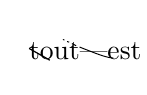
\begin{tikzpicture}[baseline=(A020G03base.base),x=0.025em,y=-0.025em]
\useasboundingbox (-2,-3) rectangle (130,53);
\node[anchor=base west,inner sep=0pt,outer sep=0pt] (A020G03base) at (0,43)
{\rlap{\unsure{tout|est}}\phantom{\deleted{\unsure{tout|est}}}};
\draw[line width=0.45pt] (0,27)--(30,44);
\draw[line width=0.35pt]
 (49,14)--(51,15)
 (55,17)--(58,18)
 (62,20)--(68,23)
 (73,25)..controls (96,34) and (110,40)..(122,41);
\end{tikzpicture}
% END R020-G05
$(n-1)+2=n+1=\operatorname{card} I+1$ (ce qui achève \unsure{aussi|ainsi} la
% A020-G04: detached high triangular point after la; source origin (565,1395).
% Shape candidate only; role, hand and surface origin unresolved. No word is in this group.
\unsure{\begin{tikzpicture}[baseline={(0,0)},x=0.025em,y=-0.025em]
\useasboundingbox (0,-33) rectangle (12,0);
\fill (4,-31)--(7,-26)--(7,-22)--(2,-24)--cycle;
\end{tikzpicture}}
\unsure{dèm.|dém.|dem.} \unsure{par|p} récurrence sur le nb des classes).

\uline{Lemme} Toute classe de $\Pi_I^\circ$ est de la forme
% B_G03: union, complete parenthesized expression, overwritten limit, raised hatted Sigma, and literal brace.
% Origin (1010,1600), 0.25 pt per source pixel, baseline y=140; fixed drawing rectangle (0,15)-(390,200).
% Pi above and X setminus to the left are outside this group. No generic bigcup or overbrace is also drawn.
$X\setminus\text{\begin{tikzpicture}[x=0.25pt,y=-0.25pt,baseline={(0,140)}]
\path[use as bounding box] (0,15) rectangle (390,200);
% U01 body; U02 upper-right loop; U03 pale lower retrace.
\draw[line width=0.95pt,line cap=round] (17,90) .. controls (17,122) and (24,140) .. (45,142) .. controls (63,142) and (72,133) .. (71,115) -- (68,87);
\draw[line width=0.55pt,line cap=round] (68,87) .. controls (66,77) and (63,81) .. (64,89) .. controls (65,96) and (68,99) .. (68,104);
\draw[black!55,line width=0.45pt,line cap=round] (19,114) .. controls (23,140) and (51,150) .. (65,133);
\node[anchor=base west,inner sep=0pt,outer sep=0pt,font=\small] at (0,190) {$\alpha\in\deleted{I}K$};
\node[anchor=base west,inner sep=0pt,outer sep=0pt,font=\small] at (91,140) {$(\Sigma_\alpha^+\cup E_\alpha)$};
\node[anchor=base west,inner sep=0pt,outer sep=0pt,font=\scriptsize] at (184,58) {$\inserted{\widehat{\Sigma}_\alpha^+}$};
% BR01 main run and central turn; BR02 closed left loop; BR03 left retrace.
\draw[line width=0.65pt,line cap=round] (108,79) .. controls (132,75) and (151,71) .. (180,74) .. controls (193,75) and (204,70) .. (217,72) -- (220,62) .. controls (234,70) and (256,68) .. (287,64) .. controls (307,60) and (326,59) .. (339,62) .. controls (344,63) and (345,66) .. (345,69);
\draw[line width=0.55pt,line cap=round] (132,76) .. controls (141,68) and (160,69) .. (164,74) .. controls (153,81) and (142,82) .. (132,76);
\draw[line width=0.85pt,line cap=round] (120,80) .. controls (145,74) and (178,73) .. (210,74);
\end{tikzpicture}}$
où $K$ est une
% G03--G04: complete insertion/cancellation/guide group with the adjoining
% words partie and de I, including the comma exactly once. No et is in it.
% Local origin full-scan (990,1755), one unit = one source pixel, y down.
% Fixed rectangle (0,0)--(420,150); baseline local y=110; base-west anchors.
\figure{\begin{tikzpicture}[x=0.018cm,y=-0.018cm,baseline={(0,110)},every node/.style={anchor=base west,inner sep=0pt,outer sep=0pt,font=\fontsize{15}{17}\selectfont}]
\path[use as bounding box] (0,0) rectangle (420,150);
\node at (11,112) {partie};
\node at (212,90) {de $I$,};
\node[rotate=10] at (161,47) {\inserted{\rlap{non vide}\phantom{\deleted{non vide}}}};
% G03: the observed oblique cancellation and its hooked right return.
\draw[line width=0.85pt,line cap=round,line join=round]
 (160,48) .. controls (204,41) and (278,23) .. (338,15)
 -- (334,11) -- (341,17)
 .. controls (337,25) and (330,31) .. (320,37);
% G04: the long curved insertion guide begins after partie and spans de I.
\draw[line width=0.7pt,line cap=round,line join=round]
 (188,99) .. controls (183,77) and (211,65) .. (253,52)
 .. controls (287,42) and (325,36) .. (355,32)
 .. controls (360,32) and (362,33) .. (362,37);
\end{tikzpicture}}
et
% slanted; the complete marginal note is in his hand.
\reversemarginpar\margin{\makebox[\linewidth][r]{\rotatebox{23}{\shortstack[l]{$K$ est $\ne\varnothing$\\si $I\ne\varnothing$}}}}\normalmarginpar
$\forall\alpha\in K$, \deleted{on a} $\Sigma_\alpha^+
% BEGIN R020-G06
% B_G05 literal relation, with A's invisible complete-state annotation method.
% Origin (943,1947), y down; baseline full y=1990.
% Full states: deleted Rightarrow followed by in | deleted to followed by in | in.
% The literal paths occur once; the first full-state candidate is primary.
\mathrel{\unsure{\text{\begin{tikzpicture}[x=0.25pt,y=-0.25pt,baseline={(0,43)}]
\path[use as bounding box] (0,0) rectangle (62,66);
\node[overlay,anchor=base west,inner sep=0pt,outer sep=0pt] at (0,43)
{\phantom{$\deleted{\Rightarrow}\in|\deleted{\to}\in|\in$}};
\draw[line width=0.70pt,line cap=round] (45,11) .. controls (35,-1) and (16,17) .. (7,32) .. controls (1,43) and (5,51) .. (15,55) .. controls (23,58) and (32,56) .. (39,51);
\draw[line width=0.75pt,line cap=round] (4,40) -- (43,32);
\draw[line width=0.40pt,line cap=round] (35,24) .. controls (38,16) and (51,29) .. (54,36) .. controls (56,34) and (54,20) .. (48,19);
\end{tikzpicture}}}}
% END R020-G06
\pi_0(X\setminus{\unsure{E|\deleted{\Sigma}E}}_\alpha)$, tels que $\forall\alpha,\beta\in K$, $\alpha\ne\beta$, on ait $\widehat{\Sigma}_\alpha^+\cap\widehat{\Sigma}_\beta^+=\varnothing$ $(\Longleftrightarrow\Sigma_\alpha^+\cap\Sigma_\beta^+=\varnothing)$.
% archive sheet number: 19
